\documentclass[aps,pre,twocolumn,10pt,nofootinbib]{revtex4-2}
\usepackage[utf8]{inputenc}
\usepackage[T1]{fontenc}
\usepackage[brazil]{babel}
\usepackage{graphicx,amsmath,booktabs,hyperref}
\graphicspath{{figuras/}}

\begin{document}
\title{Mini-projeto 01: classificação com métodos tradicionais I}
\author{Lucas Severino}
\date{\today}
\begin{abstract}
Comparamos SVM (linear e gaussiano), regressão logística e $k$ vizinhos mais
próximos em dois problemas: o indicador de diabetes do CDC (binário, 253 mil
respostas, 86\% numa classe só) e a expressão de 77 proteínas no córtex de
camundongos modelo de síndrome de Down (8 classes, 72 animais). No CDC, a
acurácia de 86\% esconde modelos que quase não detectam diabéticos; pesar as
classes eleva a revocação de 0--24\% para 65--79\%. No conjunto de proteínas,
dividir treino e teste por medição, e não por animal, infla todas as métricas
para cerca de 99\%; com a divisão correta, a regressão logística obtém o
melhor $F_1$ (0,75) e o kNN o pior (0,45).
\end{abstract}
\maketitle

Código: \url{https://github.com/lucasst28/miniprojeto01-svm-lr-knn}. Os
resultados são reproduzidos pelos notebooks \texttt{cdc.ipynb} e
\texttt{mice.ipynb}.

\section{Dados e métricas de avaliação}

\paragraph{CDC (obrigatório).}
\textit{CDC Diabetes Health Indicators} (OpenML 46841): 253\,680 respostas
ao questionário BRFSS de 2015, com 21 atributos inteiros. A maioria é
indicadora binária (hipertensão, colesterol alto, tabagismo, atividade
física...); os demais são o IMC (média 28,4, desvio 6,6) e escalas ordinais
de saúde geral, idade, escolaridade e renda. O alvo indica diabetes ou
pré-diabetes, presente em 13,9\% das respostas.

\paragraph{Mice Protein Expression (Kaggle).}
Níveis de expressão de 77 proteínas e proteínas fosforiladas medidos na
fração nuclear do córtex de 72 camundongos~\cite{higuera2015}. Parte dos
animais é trissômica (modelo Ts65Dn de síndrome de Down), o que triplica,
entre outros, o gene da proteína precursora amiloide (APP), ligado ao
Alzheimer precoce na síndrome de Down. As 8 classes combinam genótipo
(\texttt{c} controle, \texttt{t} trissômico), estímulo de aprendizado
(\texttt{CS} condicionado, \texttt{SC} não condicionado) e tratamento
(\texttt{m} memantina, \texttt{s} salina). Cada animal tem 15 medições, num
total de 1\,080 linhas, com 105 a 150 por classe. Há 1\,396 valores
faltantes (1,7\%), concentrados em poucas proteínas (BCL2 tem 26\% de
faltantes, H3MeK4 25\%), preenchidos pela mediana do treino.
A Tab.~\ref{tab:estat} resume atributos selecionados: no CDC, MentHlth e
PhysHlth têm mediana zero e variância alta; no conjunto de proteínas,
mostramos produtos de genes triplicados no modelo Ts65Dn (DYRK1A, APP,
SOD1) e duas proteínas ligadas à plasticidade sináptica (BDNF, pERK). As
escalas e caudas variam muito: DYRK1A e pERK chegam a 6 vezes a média,
enquanto APP e BDNF são concentradas, o que reforça a necessidade da
padronização.

\begin{table}[t]
\caption{Estatísticas descritivas de atributos selecionados. Expressão
das proteínas em unidades arbitrárias.}
\label{tab:estat}
\begin{ruledtabular}
\begin{tabular}{llcccc}
Base & Atributo & Média & Desvio & Variância & Mín.--Máx. \\
\hline
CDC  & BMI      & 28,38 & 6,61 & 43,68 & 12--98 \\
     & GenHlth  & 2,51  & 1,07 & 1,14  & 1--5 \\
     & MentHlth & 3,18  & 7,41 & 54,95 & 0--30 \\
     & PhysHlth & 4,24  & 8,72 & 76,00 & 0--30 \\
     & Age      & 8,03  & 3,05 & 9,33  & 1--13 \\
     & Income   & 6,05  & 2,07 & 4,29  & 1--8 \\
\hline
Mice & DYRK1A   & 0,426 & 0,249 & 0,062 & 0,15--2,52 \\
     & APP      & 0,405 & 0,061 & 0,004 & 0,24--0,63 \\
     & SOD1     & 0,543 & 0,281 & 0,079 & 0,22--1,87 \\
     & BDNF     & 0,319 & 0,049 & 0,002 & 0,12--0,50 \\
     & pERK     & 0,546 & 0,345 & 0,119 & 0,15--3,57 \\
\end{tabular}
\end{ruledtabular}
\end{table}

\paragraph{Protocolo.}
Todos os modelos usam o scikit-learn~\cite{sklearn}.
Atributos padronizados ($z$-score) dentro do \textit{pipeline}; divisão
estratificada 80/20; hiperparâmetros escolhidos por \texttt{GridSearchCV}
com validação cruzada de 5 dobras apenas no treino, maximizando o $F_1$
macro. Duas decisões dependem dos dados:
\begin{itemize}
\item \emph{Proteínas:} as colunas de genótipo, tratamento e comportamento
compõem o próprio rótulo e foram removidas. Treino, teste e dobras da
validação são separados \emph{por animal} (\texttt{StratifiedGroupKFold}):
57 camundongos no treino e 15 no teste.
\item \emph{CDC:} o SVM tem custo superlinear no número de amostras e foi
treinado numa subamostra estratificada de 20\,000 pontos; o kNN, cuja
predição percorre o treino, em 50\,000. A regressão logística usa o treino
completo (202\,944). O teste tem 50\,736 respostas para todos.
\end{itemize}

\paragraph{Por que a acurácia sozinha engana.}
O problema aparece quando comparamos a acurácia com o que o modelo faz com
a classe minoritária. No CDC, 86,1\% das respostas são de pessoas sem
diabetes; portanto, basta repetir esse rótulo em todas as previsões para
alcançar 86,1\% de acurácia. Esse resultado parece alto, mas corresponde a
revocação zero para diabetes: nenhum caso positivo é encontrado. Por isso,
também observamos precisão, revocação, $F_1$ e a matriz de confusão. No
Mice Protein, a situação é diferente: as oito classes têm proporções
próximas, e a maior reúne 13,9\% das medições. Nesse caso, usamos as
médias macro, que calculam a métrica por classe e atribuem o mesmo peso a
todas elas.

\section{Máquina de vetores de suporte}
\subsection{Sobre o método}
Uma maneira de visualizar o SVM é imaginar várias fronteiras possíveis
entre as classes e escolher aquela que deixa a maior faixa de separação em
torno dela. Para um hiperplano linear, a largura dessa faixa é a margem
$2/\lVert w\rVert$. Os exemplos que encostam nessa faixa ou ficam dentro
dela são os vetores de suporte: são eles que exercem influência direta na
posição da fronteira. Quando não é possível separar todos os pontos sem
erros, usamos a versão de margem suave,
\begin{equation}
\min_{w,b}\ \tfrac12\lVert w\rVert^2 + C\sum_i \max\bigl(0,\,1 - y_i(w^\top x_i + b)\bigr),
\end{equation}
em que $C$ determina quanto o ajuste penaliza as violações da margem. Um
$C$ maior dá mais peso a essas violações; um $C$ menor permite mais delas
em troca de uma margem potencialmente mais larga. Para representar
separações não lineares, usamos o núcleo gaussiano
$k(x,x') = \exp(-\gamma\lVert x-x'\rVert^2)$. O parâmetro
$\gamma$ define o alcance da influência de cada ponto: valores altos
produzem uma influência mais local e podem gerar fronteiras mais
irregulares; valores baixos levam a fronteiras mais suaves.

A escala das variáveis também interfere nessa geometria. No CDC, por
exemplo, o IMC varia de 12 a 98, enquanto indicadores como hipertensão
(\texttt{HighBP}) assumem apenas 0 ou 1. Sem padronização, a variação
numérica do IMC poderia dominar as distâncias usadas pelo núcleo e afetar
a margem. Por isso, o $z$-score é aplicado dentro do \textit{pipeline}.
Durante o ajuste, os parâmetros que definem a fronteira são aprendidos:
$w$ e $b$ na formulação linear, ou os multiplicadores $\alpha_i$ na
formulação dual. Já $C$ e $\gamma$ são hiperparâmetros, escolhidos por
validação cruzada, e não coeficientes aprendidos diretamente. O peso das
classes altera
ainda a penalidade dos erros: com \texttt{class\_weight=balanced}, os erros
da classe menos frequente recebem maior custo. Isso é importante no CDC,
onde o SVM linear sem pesos acabou prevendo apenas a classe majoritária.

\subsection{Experimento}
No CDC (Tab.~\ref{tab:cdc}), o SVM linear sem pesos escolhe a solução
trivial: prevê ``sem diabetes'' para todos os casos
(Fig.~\ref{fig:cdc-cm}, esquerda) e obtém 86,1\% de acurácia com $F_1 = 0$.
Com pesos balanceados, passa a encontrar 78,6\% dos diabéticos, à custa de
precisão 0,30. O núcleo gaussiano ($C=1$, $\gamma=0{,}1$) não supera o
linear no teste e mostra sobreajuste ($F_1$ 0,58 no treino e 0,42 no
teste). No conjunto de proteínas (Tab.~\ref{tab:mice}), os dois SVMs têm
$F_1 \approx 0{,}66$.

\begin{table}[t]
\caption{CDC, conjunto de teste ($n = 50\,736$). Precisão (P), revocação (R)
e $F_1$ referem-se à classe diabetes; ``bal.'' indica
\texttt{class\_weight=balanced}.}
\label{tab:cdc}
\begin{ruledtabular}
\begin{tabular}{lccccc}
Modelo & Acur. & P & R & $F_1$ & $F_1$ treino \\
\hline
Trivial (majoritária) & 0,861 & 0,000 & 0,000 & 0,000 & 0,000 \\
\hline
SVM linear          & 0,861 & 0,000 & 0,000 & 0,000 & 0,000 \\
SVM RBF             & 0,846 & 0,399 & 0,210 & 0,275 & 0,778 \\
Regressão logística & 0,862 & 0,517 & 0,158 & 0,242 & 0,244 \\
kNN ($k=3$)         & 0,837 & 0,367 & 0,237 & 0,288 & 0,578 \\
\hline
SVM linear (bal.)   & 0,712 & 0,298 & 0,786 & 0,432 & 0,433 \\
SVM RBF (bal.)      & 0,745 & 0,305 & 0,649 & 0,415 & 0,581 \\
Reg. log. (bal.)    & 0,731 & 0,311 & 0,761 & 0,441 & 0,443 \\
\end{tabular}
\end{ruledtabular}
\end{table}

\begin{figure}[t]
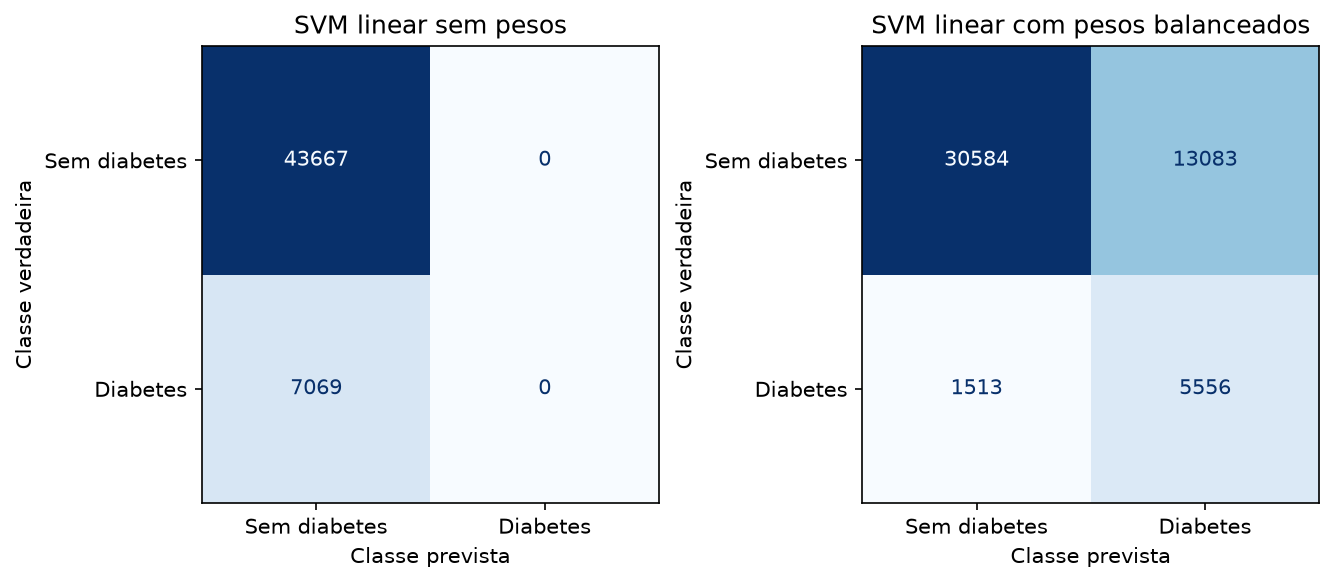
\includegraphics[width=\columnwidth]{cdc_matriz_svm_linear.png}
\caption{CDC: matriz de confusão do SVM linear sem pesos (esquerda), que
nunca prevê diabetes, e com pesos balanceados (direita).}
\label{fig:cdc-cm}
\end{figure}

\begin{figure*}[t]
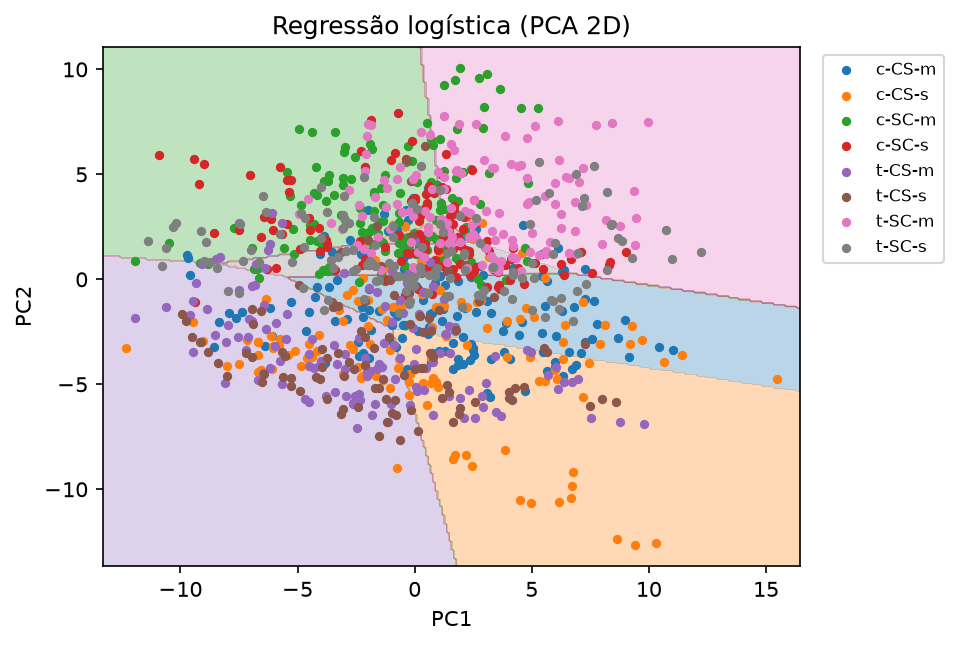
\includegraphics[width=0.49\textwidth]{mice_fronteira_lr.png}\hfill
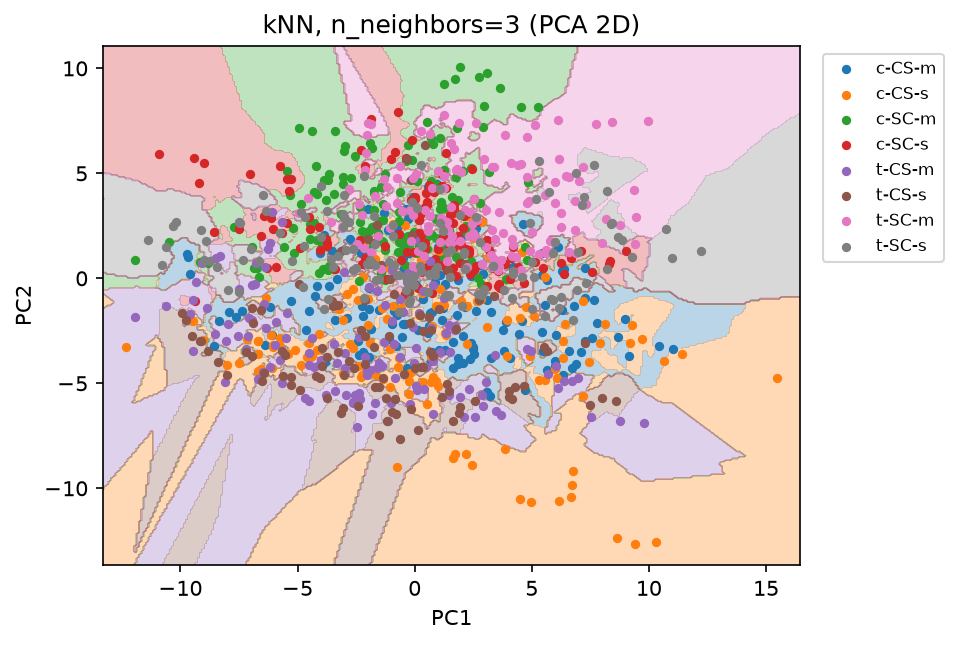
\includegraphics[width=0.49\textwidth]{mice_fronteira_knn.png}
\caption{Mice Protein: regiões de decisão da regressão logística (esquerda)
e do kNN com $k=3$ (direita), ajustados nas duas primeiras componentes
principais. As classes se sobrepõem no plano, embora sejam razoavelmente
separáveis nas 77 dimensões; o kNN produz fronteiras fragmentadas que
seguem pontos individuais.}
\label{fig:fronteira}
\end{figure*}

\section{Regressão logística}
\subsection{Sobre o método}
Na versão binária, a regressão logística representa a probabilidade da
classe positiva por
$P(y=1\mid x) = \sigma(w^\top x + b)$, com
$\sigma(z) = 1/(1+e^{-z})$. Os parâmetros são estimados a partir dos dados
minimizando a entropia cruzada,
\begin{equation}
\mathcal{L} = -\sum_i \bigl[y_i \log p_i + (1-y_i)\log(1-p_i)\bigr]
+ \tfrac{1}{2C}\lVert w\rVert^2 ,
\end{equation}
em que $p_i = \sigma(w^\top x_i + b)$ é a probabilidade estimada para a
classe positiva na amostra $i$. O segundo termo é a regularização L2: ele
penaliza coeficientes muito altos, e $C$ controla sua intensidade (valores
menores significam regularização mais forte). Assim, a função de perda
ajusta os pesos para prever as probabilidades, enquanto a regularização
limita a complexidade do modelo.

Para várias classes, a mesma ideia é estendida pelo softmax: o modelo
produz um escore $z_k$ para cada classe e os converte em probabilidades,
$P(y=k\mid x) = e^{z_k/T}/\sum_j e^{z_j/T}$, em que
$z_k = w_k^\top x + b_k$. Com duas classes, o softmax com temperatura $T$
equivale a $\sigma((z_1-z_0)/T)$; para $T=1$, reduz-se a
$\sigma(z_1-z_0)$, isto é, à regressão logística binária. O parâmetro $T$
é a temperatura: valores baixos concentram a probabilidade na classe de
maior escore, enquanto valores altos deixam a distribuição mais uniforme.
Para qualquer $T$ positivo, a ordem dos escores não muda e, portanto, a
classe de maior probabilidade permanece a mesma; no limite $T\to 0$, a
distribuição se aproxima de uma escolha pelo argmax~\cite{d2l}.

\subsection{Experimento}
No CDC, sem pesos, tem a maior acurácia (0,862), mas classifica como
saudáveis 5\,950 dos 7\,069 diabéticos do teste (revocação 0,158). Com
pesos balanceados e regularização forte ($C=0{,}01$), obtém o melhor $F_1$
(0,441), empatada na prática com o SVM linear, e as métricas de treino e
teste coincidem: não há sobreajuste.

No conjunto de proteínas é o melhor modelo ($F_1 = 0{,}749$,
Fig.~\ref{fig:mice}). Os erros se concentram entre classes que diferem
apenas no tratamento: 17 das 30 medições de \texttt{c-CS-m} são
classificadas como \texttt{c-CS-s}, e \texttt{t-CS-m} e \texttt{t-CS-s} se
confundem nos dois sentidos. Isso sugere que, nessas condições, a memantina
altera pouco o perfil das proteínas medidas.

\begin{table}[t]
\caption{Mice Protein, conjunto de teste (15 camundongos, 225 medições).
Métricas com média macro sobre as 8 classes. A última coluna repete o
$F_1$ com a divisão ingênua, que mistura medições do mesmo animal entre
treino e teste.}
\label{tab:mice}
\begin{ruledtabular}
\begin{tabular}{lccccc}
Modelo & Acur. & P & R & $F_1$ & $F_1$ ingênuo \\
\hline
SVM linear          & 0,724 & 0,699 & 0,679 & 0,670 & 0,996 \\
SVM RBF             & 0,724 & 0,664 & 0,679 & 0,659 & 0,996 \\
Regressão logística & 0,773 & 0,798 & 0,762 & 0,749 & 0,986 \\
kNN ($k=3$)         & 0,502 & 0,452 & 0,471 & 0,451 & 0,991 \\
\end{tabular}
\end{ruledtabular}
\end{table}

\begin{figure}[t]
\centering
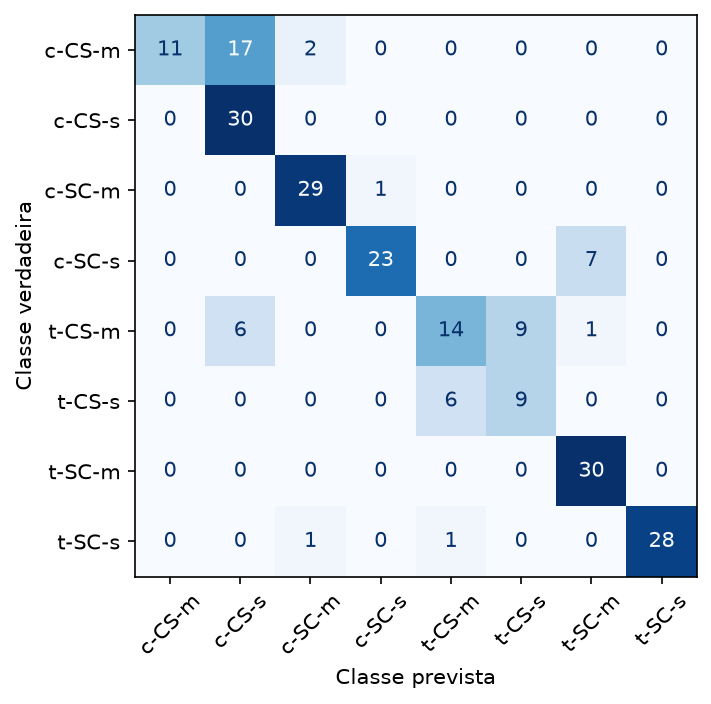
\includegraphics[width=0.78\columnwidth]{mice_matriz_lr.png}
\caption{Mice Protein: matriz de confusão da regressão logística no teste.}
\label{fig:mice}
\end{figure}

\section{$k$ vizinhos mais próximos}
\subsection{Sobre o método}
No kNN, a decisão é tomada consultando os próprios exemplos já observados:
para classificar uma nova amostra, calculamos sua distância até os pontos
do treino e escolhemos a classe mais frequente entre os $k$ mais próximos.
Diferentemente dos outros métodos deste relatório, não se estima uma
fronteira por meio de coeficientes durante o ajuste; a etapa de treino
basicamente armazena as observações e seus rótulos. O trabalho maior fica
para cada previsão, pois é necessário comparar a nova amostra com os dados
armazenados.

Como a regra depende de distâncias, a unidade de medida de cada atributo
pode mudar quem aparece como vizinho. No CDC, por exemplo, o IMC ocupa uma
faixa numérica bem maior do que um indicador binário como \texttt{HighBP};
sem padronizar, o IMC poderia ter influência desproporcional na distância.
A padronização reduz esse efeito. Ainda assim, muitas dimensões podem
atrapalhar: em espaços de dimensão elevada, as distâncias entre pontos
ficam menos contrastantes e os vizinhos próximos perdem poder de
discriminação, fenômeno conhecido como maldição da dimensionalidade~\cite{beyer1999}.
Isso é relevante no Mice Protein, que tem 77 proteínas por amostra e no
qual o kNN obteve o menor $F_1$ de teste (0,451); testamos essa explicação
na Seção~V.

\subsection{Experimento}
A validação cruzada escolheu $k=3$ nos dois conjuntos. A
Tab.~\ref{tab:knn} mostra as métricas no treino, pedidas no enunciado, ao
lado das de teste: no CDC, $F_1$ 0,58 contra 0,29; no conjunto de
proteínas, praticamente 1,0 contra 0,45.

\begin{table}[t]
\caption{kNN ($k=3$): métricas no conjunto de treino e no de teste. No CDC,
o treino é a subamostra de 50\,000 pontos e as métricas referem-se à classe
diabetes; no Mice Protein, médias macro.}
\label{tab:knn}
\begin{ruledtabular}
\begin{tabular}{llcccc}
Base & Conjunto & Acur. & P & R & $F_1$ \\
\hline
CDC  & treino & 0,903 & 0,735 & 0,476 & 0,578 \\
     & teste  & 0,837 & 0,367 & 0,237 & 0,288 \\
\hline
Mice & treino & 0,999 & 0,999 & 0,999 & 0,999 \\
     & teste  & 0,502 & 0,452 & 0,471 & 0,451 \\
\end{tabular}
\end{ruledtabular}
\end{table} Com $k$ pequeno, cada
ponto de treino conta como vizinho de si mesmo, então o desempenho de
treino não mede generalização. O kNN não tem pesos por classe e não se
beneficia do balanceamento no CDC.

O kNN é também o que mais revela o vazamento no conjunto de proteínas. Com
a divisão ingênua, a validação escolhe $k=1$ e o $F_1$ chega a 0,991: o
vizinho mais próximo de uma medição é outra réplica do mesmo animal, não um
animal com o mesmo perfil. Com a divisão por animal, ele é o pior modelo,
pois em 77 dimensões as distâncias euclidianas entre animais diferentes são
pouco discriminativas.

\paragraph{Fronteiras.}
Para desenhar as regiões de decisão, projetamos os dados nas duas primeiras
componentes principais e reajustamos cada modelo nesse plano
(Fig.~\ref{fig:fronteira}). A projeção perde a maior parte da informação,
por isso as figuras ilustram a forma das fronteiras (lineares na regressão
logística e no SVM linear, curvas no RBF, fragmentadas no kNN), e não o
desempenho dos modelos. As figuras de todos os modelos estão no repositório.

\section{Análise das proteínas}

Três experimentos adicionais no conjunto de proteínas, todos com a mesma
divisão e a mesma validação cruzada por animal
(Fig.~\ref{fig:ext}, Tab.~\ref{tab:ext}).

\begin{figure*}[t]
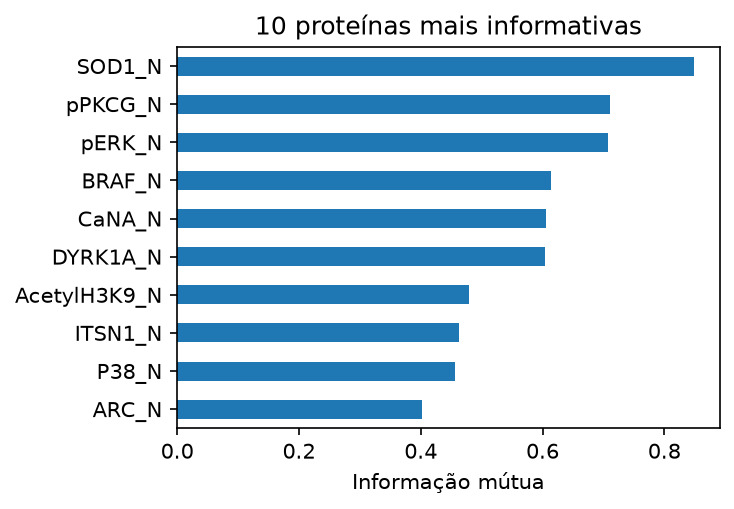
\includegraphics[width=0.32\textwidth]{mice_informacao_mutua.png}\hfill
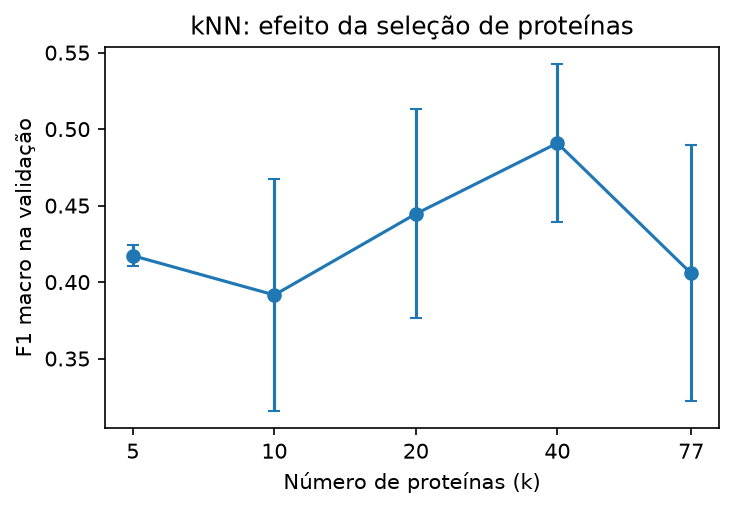
\includegraphics[width=0.32\textwidth]{mice_knn_selecao.png}\hfill
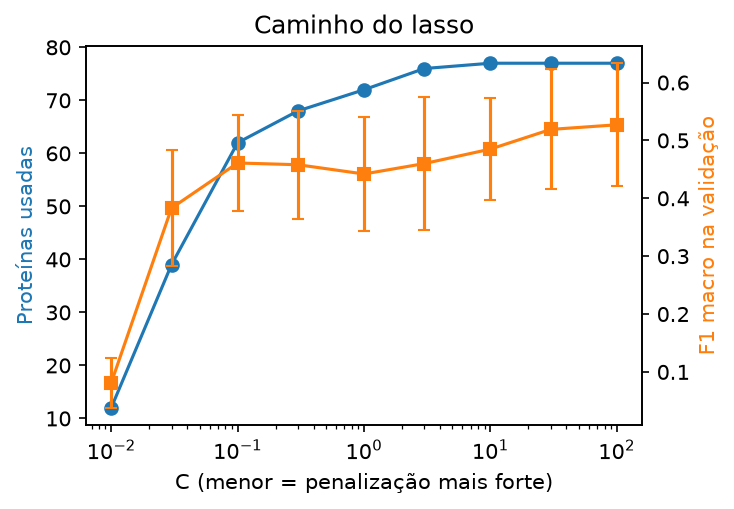
\includegraphics[width=0.32\textwidth]{mice_lasso.png}
\caption{Mice Protein. Esquerda: informação mútua de cada proteína com a
classe, calculada só no treino (10 maiores). Centro: $F_1$ de validação do
kNN em função do número de proteínas escolhidas por informação mútua
dentro do \textit{pipeline} (melhor número de vizinhos para cada ponto).
Direita: caminho do lasso; número de proteínas com peso não nulo (azul) e
$F_1$ de validação (laranja) em função de $C$. Barras: desvio entre
as 5 dobras.}
\label{fig:ext}
\end{figure*}

\paragraph{Proteínas mais informativas.} A informação mútua com a classe
coloca no topo SOD1 (0,85), pPKCG, pERK, BRAF, CaNA e DYRK1A (0,60). Duas
delas, SOD1 e DYRK1A, são produtos de genes triplicados no modelo Ts65Dn,
o que dá sentido biológico ao ranking: o genótipo deixa uma marca direta
no nível dessas proteínas.

\paragraph{kNN com seleção de atributos.} Para testar se as 77 dimensões
prejudicam o kNN, incluímos um \texttt{SelectKBest} por informação mútua
dentro do \textit{pipeline}, ajustado a cada dobra para não vazar
informação. Com 40 proteínas, o $F_1$ de validação sobe de 0,406 para
0,491, e o de teste, de 0,451 para 0,495. A curva não é monotônica e os
desvios entre dobras são grandes, mas o resultado apoia a explicação da
Seção~IV: parte das proteínas só acrescenta ruído às distâncias. Mesmo
assim, o kNN continua bem abaixo dos modelos lineares.

\paragraph{Regressão logística com lasso.} A penalização L1 zera pesos e
poderia selecionar um subconjunto pequeno de proteínas. O caminho do lasso
mostra o contrário: reduzir para 39 proteínas derruba o $F_1$ de validação
para 0,38, e o melhor valor (0,527) aparece com regularização fraca e todas
as 77 proteínas, empatado com a penalização L2 (0,535). A informação está
espalhada por muitas proteínas. O contraste com o kNN é instrutivo: a
regressão logística já pode dar peso pequeno às proteínas irrelevantes,
enquanto o kNN as soma com o mesmo peso na distância.

\begin{table}[t]
\caption{Extensões no Mice Protein: $F_1$ macro da validação (média
$\pm$ desvio) e do teste. As regressões logísticas usam o solver
\texttt{saga} e uma grade de $C$ estendida; por isso a L2 difere
ligeiramente da Tab.~\ref{tab:mice}.}
\label{tab:ext}
\begin{ruledtabular}
\begin{tabular}{lccc}
Modelo & Proteínas & $F_1$ VC & $F_1$ teste \\
\hline
kNN, todas ($k=3$)         & 77 & $0{,}406 \pm 0{,}084$ & 0,451 \\
kNN + seleção ($k=5$)      & 40 & $0{,}491 \pm 0{,}051$ & 0,495 \\
Reg. logística L2 ($C=3$)   & 77 & $0{,}535 \pm 0{,}102$ & 0,732 \\
Reg. logística L1 ($C=100$) & 77 & $0{,}527 \pm 0{,}106$ & 0,706 \\
\end{tabular}
\end{ruledtabular}
\end{table}

\section{Comparação}

\begin{figure*}[t]
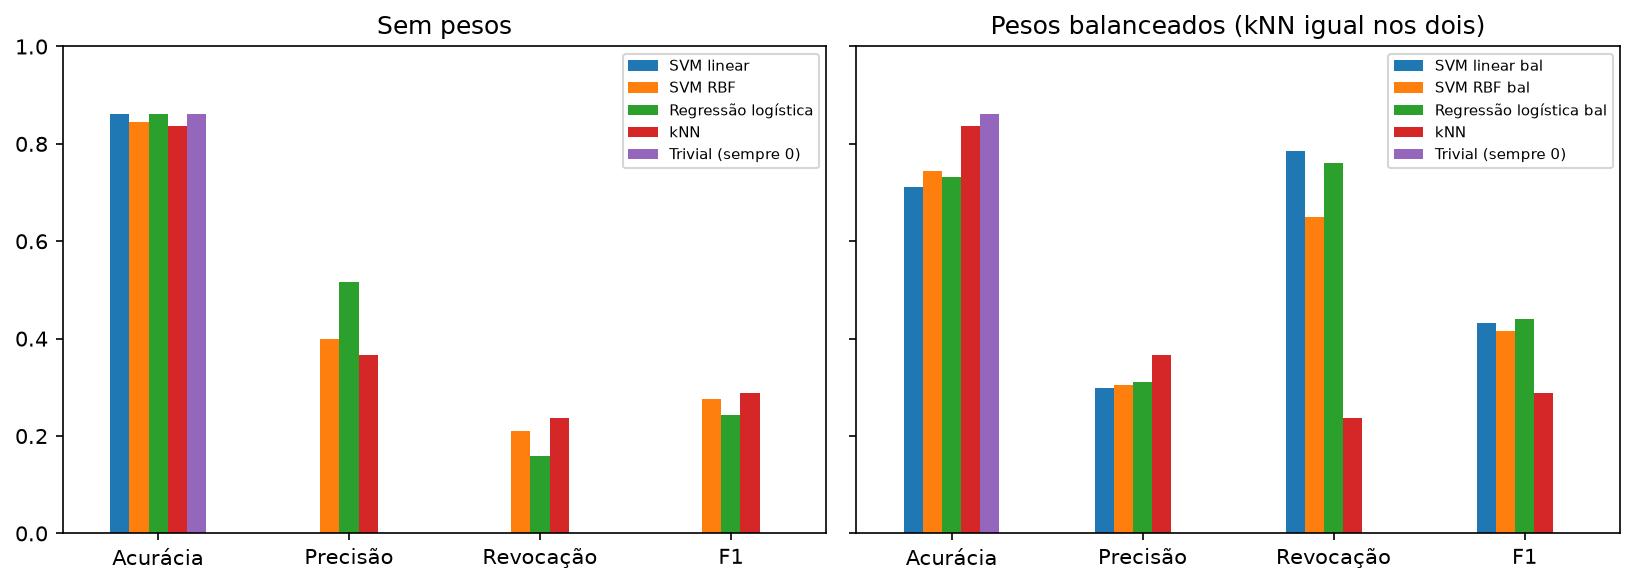
\includegraphics[width=0.6\textwidth]{cdc_painel.png}\hfill
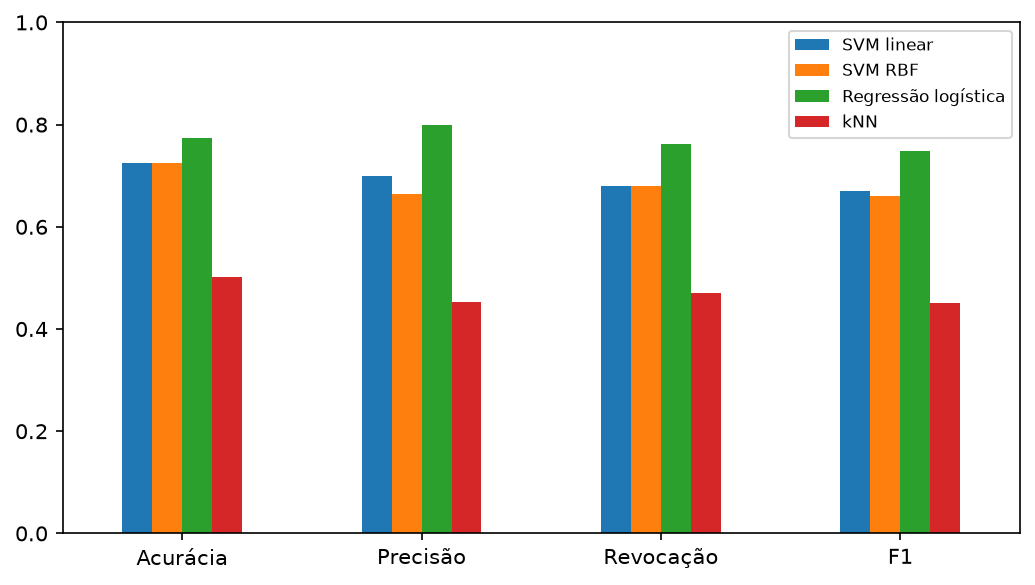
\includegraphics[width=0.38\textwidth]{mice_painel.png}
\caption{Painel comparativo: métricas no conjunto de teste de todos os
modelos. Esquerda: CDC sem pesos e com pesos balanceados, com a referência
trivial que sempre responde ``sem diabetes''; as métricas referem-se à
classe diabetes. Direita: Mice Protein (divisão por animal), médias macro.}
\label{fig:painel}
\end{figure*}

\begin{table*}[t]
\caption{Hiperparâmetros escolhidos, $F_1$ macro da validação cruzada
(média $\pm$ desvio entre as 5 dobras), $F_1$ de teste com intervalo de
confiança de 95\% por \textit{bootstrap}~\cite{efron1993} (1\,000
reamostragens) e intervalo
da diferença de $F_1$ em relação ao melhor modelo (\textit{bootstrap}
pareado; se não contém zero, a diferença é significativa). No CDC (modelos
com pesos), o $F_1$ de teste é o da classe diabetes e o valor-$p$ é do teste
exato de McNemar~\cite{mcnemar1947} contra o melhor modelo. No Mice Protein, o
\textit{bootstrap} sorteia animais e o McNemar não se aplica (n.a.), pois
as medições de um mesmo animal não são independentes.}
\label{tab:sig}
\begin{ruledtabular}
\begin{tabular}{llcccccc}
Base & Modelo & Hiperparâmetros & $F_1$ VC & $F_1$ teste & IC 95\% & IC 95\% da diferença & $p$ McNemar \\
\hline
CDC  & SVM linear          & $C=1$                    & $0{,}620 \pm 0{,}008$ & 0,432 & [0,425; 0,440] & [$-0{,}011$; $-0{,}007$] & $<10^{-4}$ \\
     & SVM RBF             & $C=1$, $\gamma=0{,}1$    & $0{,}631 \pm 0{,}005$ & 0,415 & [0,407; 0,424] & [$-0{,}032$; $-0{,}021$] & $<10^{-4}$ \\
     & Regressão logística & $C=0{,}01$               & $0{,}633 \pm 0{,}002$ & 0,441 & [0,434; 0,449] & melhor & -- \\
     & kNN                 & $k=3$                    & $0{,}593 \pm 0{,}003$ & 0,288 & [0,277; 0,299] & [$-0{,}165$; $-0{,}142$] & $<10^{-4}$ \\
\hline
Mice & SVM linear          & $C=0{,}1$                & $0{,}549 \pm 0{,}093$ & 0,670 & [0,473; 0,881] & [$-0{,}190$; $0{,}058$]  & n.a. \\
     & SVM RBF             & $C=10$, $\gamma=0{,}01$  & $0{,}552 \pm 0{,}054$ & 0,659 & [0,487; 0,878] & [$-0{,}217$; $0{,}076$]  & n.a. \\
     & Regressão logística & $C=1$                    & $0{,}535 \pm 0{,}106$ & 0,749 & [0,588; 0,900] & melhor & n.a. \\
     & kNN                 & $k=3$                    & $0{,}406 \pm 0{,}084$ & 0,451 & [0,286; 0,647] & [$-0{,}434$; $-0{,}142$] & n.a. \\
\end{tabular}
\end{ruledtabular}
\end{table*}

A Fig.~\ref{fig:painel} reúne as métricas de teste de todos os modelos, e a
Tab.~\ref{tab:sig}, os testes de significância.

\paragraph{CDC.} Com pesos balanceados, a regressão logística tem o maior
$F_1$ (0,441). Como o teste tem 50\,736 casos, até diferenças pequenas são
estatisticamente detectáveis: o intervalo da diferença para o SVM linear
($-1{,}1$ a $-0{,}7$ ponto) não contém zero e o McNemar dá $p<10^{-4}$. A
diferença é significativa, mas irrelevante na prática. O kNN fica 14 a 16
pontos abaixo. A regressão logística é preferível: treina em cerca de 2~s
no conjunto completo, contra 47 a 68~s do SVM numa subamostra de 10\%, e
não sobreajusta. Em nenhum caso um modelo vai muito além de
$F_1 \approx 0{,}44$, o que sugere que os 21 atributos do questionário
carregam informação limitada sobre o diagnóstico.

\paragraph{Proteínas.} A unidade amostral é o animal, não a medição. Com 15
animais no teste, um único animal mal classificado move a acurácia em cerca
de 6,7 pontos, e os intervalos de confiança são largos (cerca de 0,4 de
amplitude). A vantagem da regressão logística sobre os SVMs não é
significativa: os intervalos da diferença contêm zero, e na validação
cruzada os três ficam entre 0,535 e 0,552, com desvio de 0,05 a 0,11 entre
as dobras. Já o kNN é significativamente pior (intervalo da diferença de
$-0{,}43$ a $-0{,}14$). A lição principal é metodológica: a divisão ingênua
faria todos os modelos parecerem quase perfeitos.

\paragraph{Limitações.} Usamos uma única divisão entre treino e teste, e o
``melhor'' modelo foi identificado no próprio teste; no Mice Protein, com
15 animais no teste, outra divisão poderia mudar a ordem entre regressão
logística e SVMs. No CDC, SVM e kNN foram ajustados em subamostras. As
fronteiras são desenhadas em duas componentes principais e não representam
a fronteira real em alta dimensão. Validação cruzada aninhada por animal
daria estimativas mais estáveis.

\section{Conclusão}
Os dois conjuntos ilustram armadilhas opostas. No CDC, o desbalanceamento
faz a acurácia recompensar modelos que ignoram a classe de interesse;
pesar as classes troca acurácia por revocação, o que é desejável numa
triagem. No conjunto de proteínas, medições repetidas do mesmo animal fazem
a avaliação medir memória, não generalização. Em ambos, o modelo linear
mais simples, a regressão logística, foi o melhor ou empatou com o melhor.
Entre as proteínas, as mais informativas incluem produtos de genes
triplicados (SOD1, DYRK1A); selecionar proteínas ajuda o kNN, mas não a
regressão logística, porque a informação está distribuída por muitas
delas.

\begin{thebibliography}{6}
\bibitem{higuera2015} C. Higuera, K. J. Gardiner e K. J. Cios,
``Self-organizing feature maps identify proteins critical to learning in a
mouse model of Down syndrome'', \textit{PLoS ONE} \textbf{10}, e0129126
(2015).
\bibitem{sklearn} F. Pedregosa \textit{et al.}, ``Scikit-learn: machine
learning in Python'', \textit{J. Mach. Learn. Res.} \textbf{12}, 2825
(2011).
\bibitem{d2l} A. Zhang, Z. C. Lipton, M. Li e A. J. Smola,
\textit{Dive into Deep Learning} (Cambridge University Press, 2023).
\bibitem{beyer1999} K. Beyer, J. Goldstein, R. Ramakrishnan e U. Shaft,
``When is `nearest neighbor' meaningful?'', em \textit{Int. Conf. on
Database Theory} (Springer, 1999), p. 217.
\bibitem{efron1993} B. Efron e R. J. Tibshirani, \textit{An Introduction
to the Bootstrap} (Chapman \& Hall, 1993).
\bibitem{mcnemar1947} Q. McNemar, ``Note on the sampling error of the
difference between correlated proportions or percentages'',
\textit{Psychometrika} \textbf{12}, 153 (1947).
\end{thebibliography}

\end{document}
